\documentclass{beamer}
\usepackage[utf8]{inputenc}
\usepackage[french]{babel}
\usepackage{pgf}
\usepackage{xcolor}  
\usepackage{graphicx}
\usepackage{colortbl}
\usepackage{wrapfig}
\usepackage{multimedia}
\usepackage{pifont}
\setbeamercolor*{Title bar}{fg=black}
\setbeamercolor*{Location bar}{fg=black}
\setbeamercolor*{frametitle}{parent=Title bar}
\setbeamercolor*{block body}{bg=white,fg=black}
\setbeamercolor*{normal text}{bg=white,fg=black}
\setbeamercolor*{section in head/foot}{bg=white,fg=black}%Couleur de la liste de navigation

\newcommand{\cmark}{\ding{51}}
\newcommand{\xmark}{\ding{55}}
\definecolor{vertFleche}{rgb}{0.20,0.43,0.09} % vert moyen
\usetheme{Normal}


\title{Présentation RPG}
\author{GUINGOIN Sylvain \\PATTYN Maxime \\RIVOIRE Claire \\SASSOULAS Pierre}

\AtBeginSection[]
{
  \begin{frame}
    \frametitle{Plan}
    \tableofcontents[currentsection]
  \end{frame}
}

\begin{document}
\frame{\titlepage}
\author{}
\frame{\tableofcontents}

\author{SASSOULAS Pierre}
\section{Introduction}
\begin{frame}
  \frametitle{Objectifs du projet}
    \begin{itemize}
        \item Jeux de rôle
        \item Personnages virtuels autonomes
        \item Scénario adaptatif 
        \item Interface graphique minimale
        \item Code modulaire pour les futurs ASI5
    \end{itemize} 
\end{frame}

\begin{frame}
  \frametitle{Réalisation}
    \begin{itemize}
        \item Positionnement, déplacement, inventaire \only<2>{\textcolor{vertFleche}{\LARGE \cmark{}}  \textit{\small} }
        \item Interaction entre et avec les PNJ \only<2>{\textcolor{vertFleche}{\LARGE \cmark{}} \textit{\small }}
        \item Objectifs priorisés comportant des étapes \only<2>{\textcolor{vertFleche}{\LARGE \cmark{}} \textit{\small }}
        \item Re-planification du scénario \only<2>{\textcolor{vertFleche}{\LARGE \cmark{}} \textit{\small }}
        \item Connaissances sur le monde \only<2>{\textcolor{vertFleche}{\LARGE \cmark{}} \textit{\small }}
        \item Distance d'interaction  \only<2>{\textcolor{red}{\LARGE \xmark{}} \textit{\small }}
        \item Lien avec le programme de Quentin \only<2>{\textcolor{red}{\LARGE \xmark{}} \textit{\small }}
    \end{itemize} 
\end{frame}

\section{Monde et environnement}
\begin{frame}
    \frametitle{Le monde}
    \begin{itemize}
        \item Monde contenant des entités (Voir AsiAventure)
        \item Lois du monde provenant de D\&D
        \item Différents types de terrain, et gestion des zones
        \item Personnages ayant des connaissances sur leur monde
    \end{itemize} 
\end{frame}

\begin{frame}
      \frametitle{Les personnages}
    \begin{itemize}
        \item Classe mère abstraite de PNJ et Joueur
        \item Caractéristiques provenant de D\&D
        \item États provenant de D\&D
        \item Gestion du sexe
        \item Implémentation de l'intelligence dans un premier temps
        \item Désirs
    \end{itemize} 
\end{frame}

\begin{frame}
      \frametitle{Actions possibles pour les personnages}
    \begin{itemize}
        \item Actions limitées ou favorisées par une caractéristique
        \item Se déplacer dans le monde
        \item Chercher une entité dans une zone
        \item Analyser un objet
        \item Analyser une zone
        \item Interroger un autre personnage
    \end{itemize} 
\end{frame}

\begin{frame}
    \frametitle{Interaction avec un autre personnage}
      \begin{itemize}
          \item Discussion sans intérêt
          \item Poser des questions à propos d'une entité
          \item Demander un objet gentiment
          \item Tuer
          \item Récupérer les objets sur le corps
      \end{itemize} 
\end{frame}

\author{GUINGOIN Sylvain}
\section{IA et gestion des entités}


\begin{frame}
  \frametitle{IA des PNJs}
  Fonctionnement des PNJs :
  \begin{itemize}
  \item Observer autour d'eux
  \item Choisir une action
  \item Effectuer cette action
  \end{itemize}
  ~\\  
  \onslide<2>{
    Implémentation sous forme de BDI : 
    \begin{itemize}
    \item Connaissances
    \item Désirs et plan d'action
    \item Actions
    \end{itemize}
  }
\end{frame}

\begin{frame}
  \frametitle{IA des PNJs}
  Les connaissances :
  \begin{itemize}
  \item Fait
  \item Position
  \item Possession
  \end{itemize}
  ~\\
  \onslide<2->{
    Les désirs sont des listes d'actions
    ~\\
    2 désirs possibles :
    \begin{itemize}
    \item Possession : ramasser des objets
    \item Connaissance : parler avec tout le monde
    \end{itemize}
    Si aucun désir réalisable : exploration du monde
  }
\end{frame}

\begin{frame}
  \frametitle{IA des PNJs}
  Les actions :
  \begin{itemize}
  \item Méthode à exécuter sur le PNJ
  \item Paramètres de la méthode
  \item Représenté en chaine de caractère
  \item Appel de la méthode par introspection
  \end{itemize}
\end{frame}


\begin{frame}
  \frametitle{Gestion des entités}
  Classe \textbf{DatabaseManager} : Injection de dépendances
  \begin{itemize}
  \item Stockage de l'ensemble des entités
  \item Récupération à partir d'un id
  \item Recherche à partir d'un ou plusieurs attributs
  \item Création d'objet ou recherche d'entité ``from String''
  \end{itemize}
\end{frame}

\author{RIVOIRE Claire}



\section{Interface graphique}

\begin{frame}

   \frametitle{Représentation du monde}
 \begin{columns}[t]
  \begin{column}{5cm}
\textbf{4 types de terrain} \\
\vspace{5mm} 
\begin{itemize}
 \item  Herbe  ~\\
\vspace{5mm} 
 \item   Terre ~ \\
\vspace{5mm} 
 \item  Forêt ~ \\
\vspace{5mm} 
 \item  Montagne 
\end{itemize}
  \end{column}
  
  \begin{column}{5cm}
\textbf{3 entités}
\vspace{5mm} 
\begin{itemize}
 \item  Objet ~ \\
\vspace{5mm} 
 \item  PNJ ~ \\
\vspace{5mm} 
 \item Joueur 
\end{itemize}

  \end{column}
 \end{columns}


  \begin{picture}(0,0)
    \put(70, 92){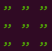
\includegraphics[scale=0.5]{./images/screenshootHerbe.png}}
  \end{picture}	
  \begin{picture}(0,0)
    \put(66, 60){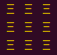
\includegraphics[scale=0.47]{./images/screenshootTerre.png}}
  \end{picture}	
  \begin{picture}(0,0)
    \put(62,27){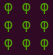
\includegraphics[scale=0.5]{./images/screenshootForet.png}}
  \end{picture}	
  \begin{picture}(0,0)
    \put(58,-4){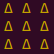
\includegraphics[scale=0.5]{./images/screenshootMontagne.png}}
  \end{picture}	

  \begin{picture}(0,0)
    \put(210, 107){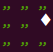
\includegraphics[scale=0.5]{./images/screenshootObjet.png}}
  \end{picture}	
  \begin{picture}(0,0)
    \put(206, 75){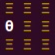
\includegraphics[scale=0.47]{./images/screenshootPNJ.png}}
  \end{picture}	
  \begin{picture}(0,0)
    \put(202, 42){
\includegraphics[scale=0.5]{./images/screenshootJoueur.png}}
  \end{picture}	
\end{frame}

\begin{frame}
\frametitle{Représentation du monde}
\begin{figure}
    \begin{center}
      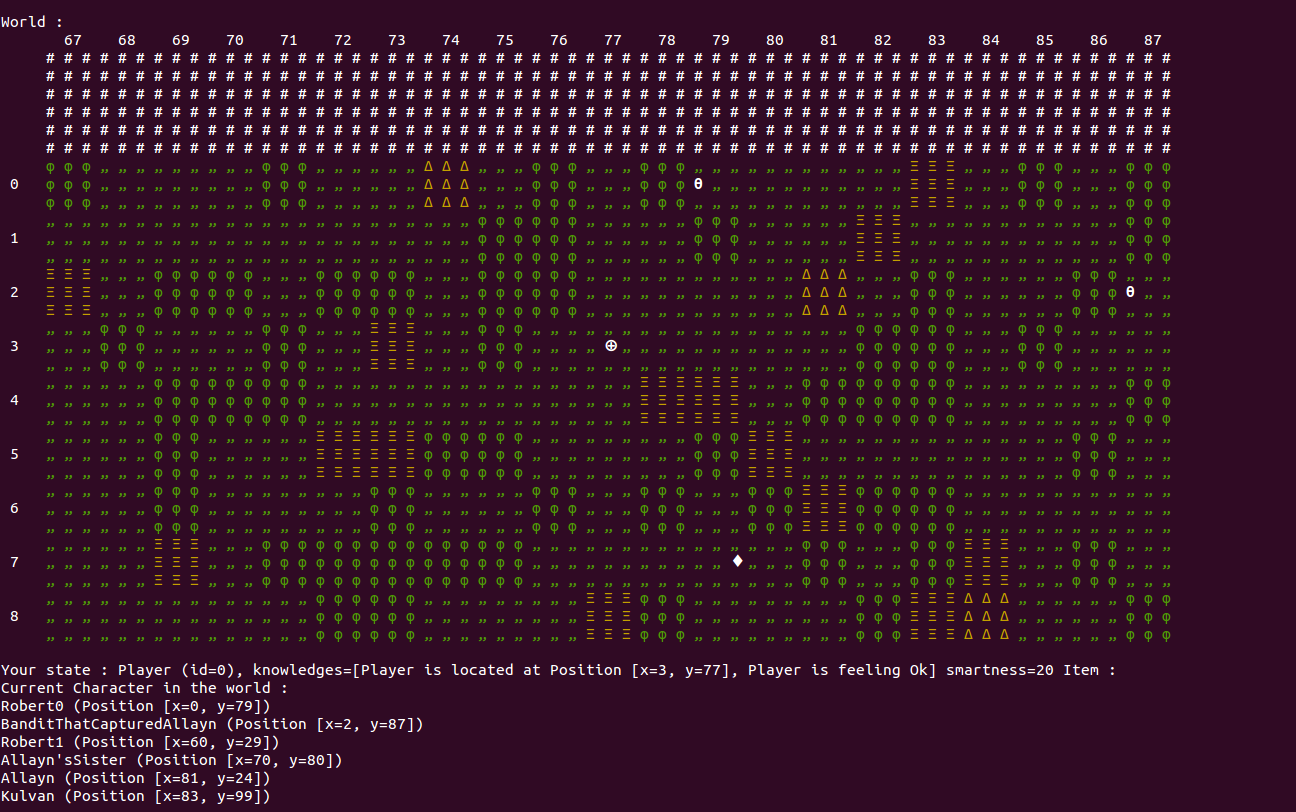
\includegraphics[scale=0.22]{./images/screenshootWorld.png}
      \caption{Le monde}
    \end{center}
  \end{figure}
\end{frame}


\section{Interactions utilisateur}
\begin{frame}
   \frametitle{Fonctionnement}
~\\
~\\
  \begin{itemize}
  \item En ligne de commande
  \item Présentation des possibilités
  \item Choix par mots-clés
  \end{itemize} 
\begin{figure}
    \begin{center}
      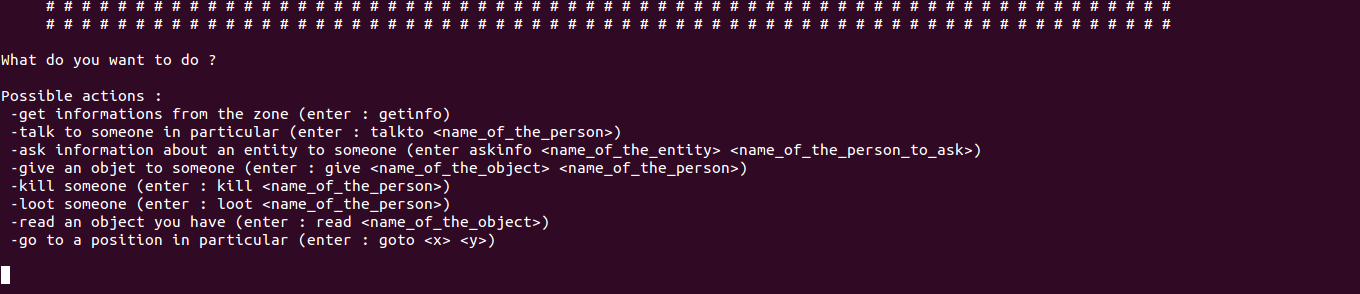
\includegraphics[scale=0.3]{./images/screenshootUI01.png}
      \caption{Exemple d'action possibles}
    \end{center}
  \end{figure}
\end{frame}

\begin{frame}
   \frametitle{Implémentation}
  \begin{itemize}
  \item Utilisation d'une classe spécifique : \textbf{UI}
  \item Séparation IHM / partie métier
  \item Messages stockés dans des constantes
  \item Mots-clés sans rapport avec les fonctions
  \end{itemize} 
\end{frame}

\author{PATTYN Maxime}

\section{Demonstration}
\begin{frame}
\begin{center}
  \textbf{Démonstration}
\end{center}
\end{frame}


\section{Conclusion}
\begin{frame}
  \frametitle{Conclusion}
  \begin{itemize}
  \item Version posant des bases solides
    \begin{itemize}
    \item Interaction simples
    \item Psychologie et Quêtes
    \end{itemize}
  \item Conception permettant une évolution future
  \item Améliorer l'aspect vivant et réaliste
    \begin{itemize}
    \item Evolution en temps réel (graphique)
    \item Quêtes évolutives
    \item PNJ plus complexes
    \end{itemize}
  \end{itemize}
\end{frame}


\end{document}
